\documentclass[11pt]{report}
\usepackage{fancyhdr}
\usepackage[utf8]{inputenc}
\usepackage[english]{babel}
\usepackage{hyperref}
\usepackage{gensymb}
\usepackage{amsmath,amssymb,amsfonts}
\usepackage{algorithmic}
\usepackage{graphicx}
\usepackage{textcomp}
\usepackage{xcolor}
\usepackage{siunitx}
\usepackage{indentfirst}
\usepackage[margin=2.5cm]{geometry}
\usepackage{float}
\usepackage[UKenglish]{datetime}
\usepackage{setspace}

\hypersetup{
    colorlinks=true,
    linkcolor=black,   
    urlcolor=blue,
}

\pagestyle{fancyplain}
\fancyhf{}
\fancyhead[R]{Student No. 10618407}
\fancyfoot[R]{\thepage}

\doublespacing

\begin{document}
\title{\bf ROCO219 - Inverted Pendulum Coursework 2020}
\author{Student No. 10618407} 								
\date{\today}
\maketitle
\pagenumbering{roman}
\setcounter{page}{2}
\tableofcontents

\chapter{Theory and Design}
\pagenumbering{arabic}

\section{State space model of the inverted pendulum}

A state space model is a useful basis for demonstrating the control of a system such as an inverted pendulum. Therefore, we implement observation based state feedback control using the augmented positional state of the cart and integral control (these are added in later). Eq.(1.1) below shows the non-linear differential equation for the inverted pendulum kinematic model.

\begin{equation}
(I + ml^2)\frac{d^2\theta}{dt^2} + \mu\frac{d\theta}{dt} = mgl sin(\theta) + ml\frac{d^2x\textsubscript{p}}{dt^2}cos(\theta)
\end{equation}

This equation can be linearised about the pendulum's unstable equilibrium point. This gives Eq.(1.2), which describes an inverted pendulum's kinematic model. 

\begin{equation}
(I + ml^2)\frac{d^2\theta}{dt^2} + \mu\frac{d\theta}{dt} = mgl\theta + ml\frac{d^2x\textsubscript{p}}{dt^2}
\end{equation}

After many derivations we can write the state space model for the inverted pendulum as shown in Eq.(1.3). This takes into account the use of velocity control on the cart to stabilise the pendulum.

\begin{equation}
\begin{bmatrix}
\dot{x}\textsubscript{1}\\
\dot{x}\textsubscript{2}\\
\end{bmatrix}
=
\begin{bmatrix}
0 && 1\\
-a\textsubscript{2} && -a\textsubscript{1}\\
\end{bmatrix}
\begin{bmatrix}
x\textsubscript{1}\\
x\textsubscript{2}\\
\end{bmatrix}
+
\begin{bmatrix}
b\textsubscript{0}\\
-a\textsubscript{1}b\textsubscript{0}
\end{bmatrix}
v\textsubscript{c}
\end{equation}

Where: 
\begin{equation}
a\textsubscript{1} = \frac{\mu}{(I + ml^2)}
\end{equation}
\begin{equation}
a\textsubscript{2} = \frac{-mgl}{(I + ml^2)}
\end{equation}
\begin{equation}
b\textsubscript{0} = \frac{ml}{(I + ml^2)}
\end{equation}

For the inverted pendulum system, we were given the required constants to create a state space model. These are as follows: 
\begin{itemize}
\item{Gravity (g) = 9.81}
\item{Length of pendulum rod (l) = 0.64m}
\item{Mass of pendulum rod (M) = 0.314kg}
\item{Coefficient of viscous friction ($\mu$) = 0.005}
\item{Moment of inertia about the center of the rod (I) = $\frac{1}{12}*M*l^2 = 0.107  kgm\textsuperscript{2}$}
\end{itemize}

For ease of calculation, the moment of inertia is considered to act about the middle of the pendulum. These constants are put into Eq.(1.4), Eq.(1.5), and Eq.(1.5). These are used to calculate a\textsubscript{1}, a\textsubscript{2}, and b\textsubscript{0}. These values are used in Eq.(1.7), Eq.(1.8), and Eq.(1.9) to calculate the values of $A$, $B$, and $C$ respectively. These can be seen in the Matlab code below:

\begin{equation}
A 
=
\begin{bmatrix}
0 & 1\\
-a\textsubscript{2} &  -a\textsubscript{1}\\
\end{bmatrix}
\end{equation}

\begin{equation}
B
=
\begin{bmatrix}
b\textsubscript{0}\\
-a\textsubscript{1}b\textsubscript{0}\\
\end{bmatrix}
\end{equation}

\begin{equation}
C
=
\begin{bmatrix}
1 & 0\\
\end{bmatrix}
\end{equation}

\begin{figure}[H]
\centerline{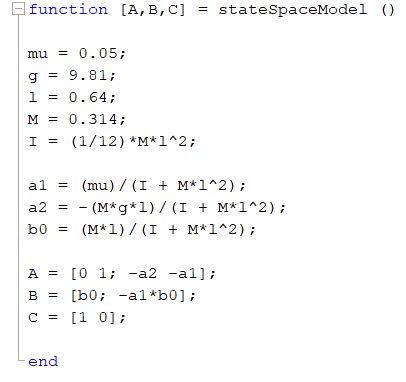
\includegraphics[width=7cm]{stateSpaceModel.png}}
\caption{Code for calculating A, B, and C in Matlab}
\label{fig}
\end{figure}

\begin{figure}[H]
\centerline{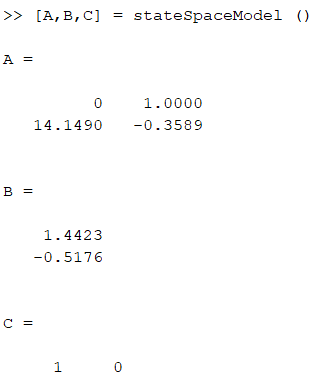
\includegraphics[width=7cm]{stateSpaceModeloutputs.png}}
\caption{Outputs A, B, and C in Matlab}
\label{fig}
\end{figure}

\section{Design a Luenberger observer to estimate state}

A Luenberger observer is used to estimate the system state of the inverted pendulum. This is done by using the state space model of the plant. To create a Luenberger observer in Matlab we use the place command along with $A$, $C'$ ($C$ transposed), and $P$. $A$ and $C$ are the matrices shown in Eq.(1.7) and Eq.(1.9) respectively. The values of $P$ are the poles of the system. $C'$ is used to swap the orientation of $C$ from a 1x2 matrix to a 2x1. This allows the place command to work as shown below:  

\begin{figure}[H]
\centerline{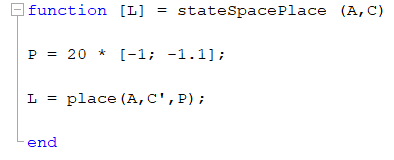
\includegraphics[width=9cm]{stateSpacePlace.png}}
\caption{Code for creating a state space place}
\label{fig}
\end{figure}

The output $L$ must be chosen such that the equation $A-LC$ yields eigenvalues with negative real parts. This causes the oscillations of the system to decay with time, making it stable. This is done by changing the poles of the system used in the place command.  The output $L$ is shown below:

\begin{figure}[H]
\centerline{\includegraphics[width=9cm]{stateSpacePlaceoutput.png}}
\caption{Output of L in Matlab}
\label{fig}
\end{figure}

\section{Augment positional state into the state space model}

Although it is possible to design a controller using just the feedback control from the 2-dimensional state derived model, in practice we want to be able to control the position of the cart. Adding an augmented positional state into the state space model is used to control the velocity of the cart. This is done to bring the cart back to a known position (usually the center of the track). This prevents the cart from moving indefinitely. The positional state stops the cart from running out of track, which would cause the pendulum to become unbalanced and fall over. To do this, a third state, x\textsubscript{3}, is added. This is used to represent the cart position. The differential of $x\textsubscript{3}$ is equal to the velocity signal as shown in Eq.(1.10):

\begin{equation}
\frac{d}{dt}(x\textsubscript{3}) = v\textsubscript{c}
\end{equation}

The new state space model for the inverted pendulum, including the augmented positional state, is shown in Eq.(1.11). The output of the system is shown in the Eq.(1.12). 

\begin{equation}
\frac{d}{dt}
\begin{bmatrix}
x\textsubscript{1}\\
x\textsubscript{2}\\
x\textsubscript{3}\\
\end{bmatrix}
=
\begin{bmatrix}
0 & 1 & 0\\
-a\textsubscript{2} & -a\textsubscript{1} & 0\\
0 & 0 & 0\\
\end{bmatrix}
\begin{bmatrix}
x\textsubscript{1}\\
x\textsubscript{2}\\
x\textsubscript{3}\\
\end{bmatrix}
+ 
\begin{bmatrix}
b\textsubscript{0}\\
-a\textsubscript{1}b\textsubscript{0}\\
1\\
\end{bmatrix}
v\textsubscript{c}
\end{equation}

\begin{equation}
y 
=
\begin{bmatrix}
1 & 0 & 0\\
\end{bmatrix}
\begin{bmatrix}
x\textsubscript{1}\\
x\textsubscript{2}\\
x\textsubscript{3}\\
\end{bmatrix}
\end{equation}

\section{Add integral action to the state space model}

Integral control is used to reduce the state space controller's steady state error. To reduce this error, another term is added into the state space controller. The added term is the integral action. This compounds the positional errors forming a larger error over time. This helps the cart return to the absolute position set using the augmented positional state. To do this, a forth state, x\textsubscript{4}, is added. The differential of $x\textsubscript{4}$ is equal to $x\textsubscript{3} - r$, as shown in Eq.(1.13). 

\begin{equation}
\frac{d}{dt}(x\textsubscript{4}) = x\textsubscript{3}-r
\end{equation}

For the inverted pendulum the value of $r$ is zero. This make the differential of $x\textsubscript{4}$ equal to the value $x\textsubscript{3}$, as shown in Eq.(1.14).

 \begin{equation}
\frac{d}{dt}(x\textsubscript{4}) = x\textsubscript{3}
\end{equation}

The new state space model, for the inverted pendulum including the integral action, is shown in Eq.(1.15). The output of the system is shown in the Eq.(1.16).

\begin{equation}
\frac{d}{dt}
\begin{bmatrix}
x\textsubscript{1}\\
x\textsubscript{2}\\
x\textsubscript{3}\\
x\textsubscript{4}\\
\end{bmatrix}
=
\begin{bmatrix}
0 & 1 & 0 & 0\\
-a\textsubscript{2} & -a\textsubscript{1} & 0 & 0\\
0 & 0 & 0 & 0\\
0 & 0 & 1 & 0\\
\end{bmatrix}
\begin{bmatrix}
x\textsubscript{1}\\
x\textsubscript{2}\\
x\textsubscript{3}\\
x\textsubscript{4}\\
\end{bmatrix}
+
\begin{bmatrix}
b\textsubscript{0}\\
-a\textsubscript{1}b\textsubscript{0}\\
1\\
0\\
\end{bmatrix}
v\textsubscript{c}
\end{equation}

\begin{equation}
y 
= 
\begin{bmatrix}
1 & 0 & 0 & 0\\
\end{bmatrix}
\begin{bmatrix}
x\textsubscript{1}\\
x\textsubscript{2}\\
x\textsubscript{3}\\
x\textsubscript{4}\\
\end{bmatrix}
\end{equation}

\section{Design a state feedback controller}

Once both augmented positional state and integral action have been added to the state space model, we can begin to design the complete state feedback controller as shown in the figures below: 

\begin{figure}[H]
\centerline{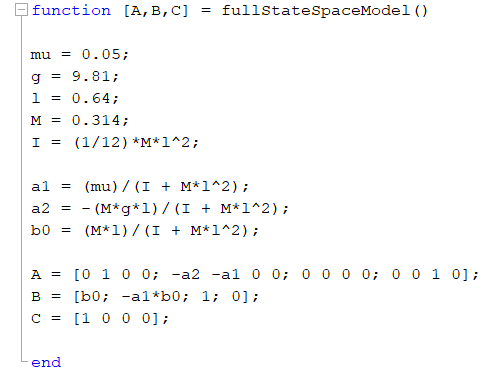
\includegraphics[width=7cm]{fullStateSpaceModel.png}}
\caption{Code for creating a full state space model}
\label{fig}
\end{figure}

\begin{figure}[H]
\centerline{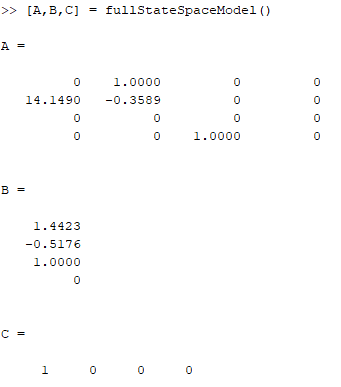
\includegraphics[width=7cm]{fullStateSpaceModeloutput.png}}
\caption{Output for A, B, and C in Matlab}
\label{fig}
\end{figure}

To implement the full feedback state controller, we need to design the feedback gain, $K$. We use the values $\hat{x}\textsubscript{1}$ and $\hat{x}\textsubscript{2}$ from the Luenberger observer. To find the eigenvalues, $\lambda$, for the state feedback control system. We use its characteristic equation, as shown in Eq.(1.17). 

\begin{equation}
|(A-BK-{\lambda}I)| = 0
\end{equation}

Using this equation, manipulating the location of the eigenvalues is straight forward. It is done by changing the value of $K$. This is done using the place command in Matlab as shown below:

\begin{figure}[H]
\centerline{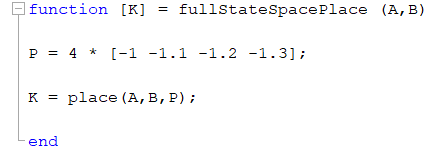
\includegraphics[width=8cm]{fullStateSpacePlace.png}}
\caption{Code for generating a full state space place}
\label{fig}
\end{figure}

\begin{figure}[H]
\centerline{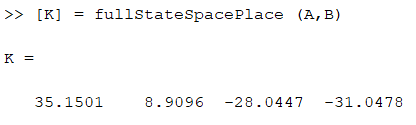
\includegraphics[width=8cm]{fullStateSpacePlaceOutput.png}}
\caption{Output for the full state space place}
\label{fig}
\end{figure}


\chapter{Implementation and Simulation}

\section{Implement the controller system using Euler integration}

The implementation of the controller system, using Euler integration, uses three main sections of code to control the pendulum. The main control program, the state space integrator, and VCPendDotCB. These are all outlined below.  

\subsection{Main Control Program}

The main control program runs through three main stages. The first stage is variable initialisation. The second stage is the main loop used to calculate the control values using the state space integrator. The third stage is used to plot the values calculated in the loop to use as an output animation for the pendulum.

\subsubsection{Variable Initialisation}

The variable initialisation starts by closing all of the open figures, clearing all of the values stored in the program and clearing the command window. This is done primarily for reassurance that the code is self contained and doesn't run any variables that may have been previously stored. This ensures a clean work space every time the program is run. 
The time points dictate how long each of the runs of the pendulum will be.

The variables for the simulation are setup. These values are the same as previously used to calculate the Lunberger observer and the state feedback gain. The values of $a\textsubscript{1}$, $a\textsubscript{2}$, and $b\textsubscript{0}$ are calculated. The transmission matrix, $D$, is initialised as a 4x1 matrix with all zeros. Although this could have been set up using a single value, 0, setting $D$ as a matrix allows you to change the values quickly. $L$ is then calculated, using a basic state space model of the inverted pendulum as in figures 1.3 and 1.4. $K$ is calculated using a full state feedback controller, incorporating augmented positional state and integral action, as in fig.(1.7) and fig.(1.8). The arrays xData, yData, tData, and kickFlag are also initialised. 

\begin{figure}[H]
\centerline{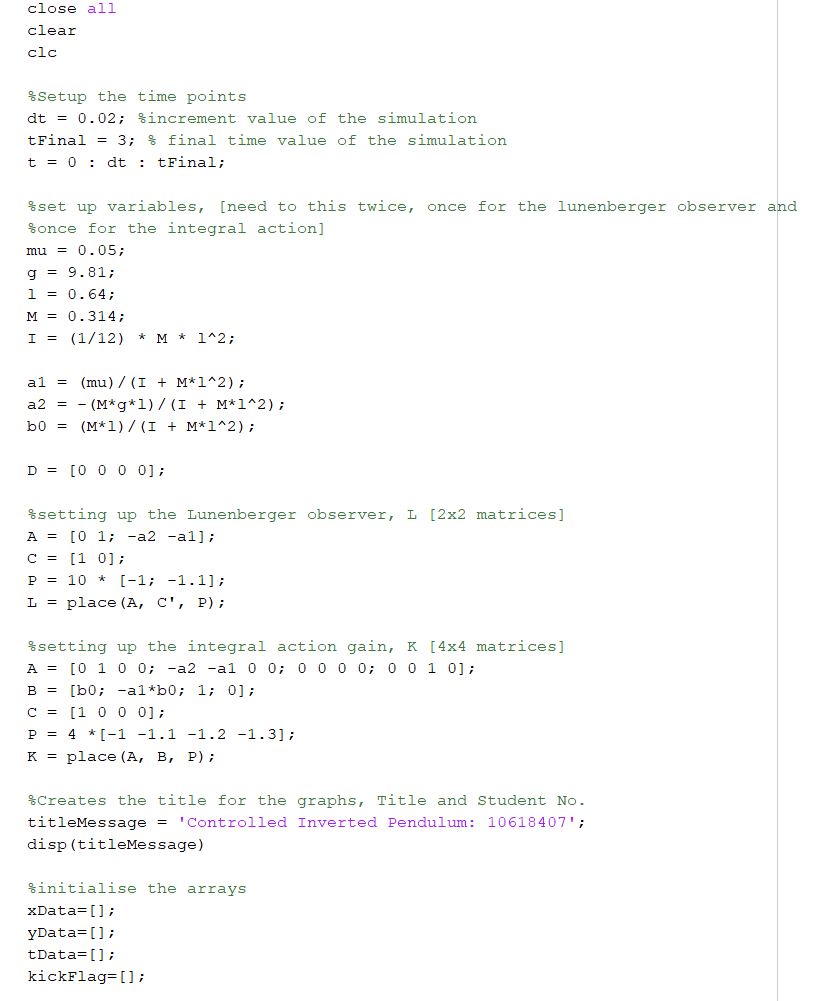
\includegraphics[width=12cm]{initMain.png}}
\caption{Initialisation of the parameters for the inverted pendulum}
\label{fig}
\end{figure} 

Setting the poles is important in controlling the motion of the pendulum. When using the poles shown in the initialisation code the pendulum is under control. The pendulum returns to its equilibrium position within one oscillation. This is known as critical damping and is shown in the graph below:

\begin{figure}[H]
\centerline{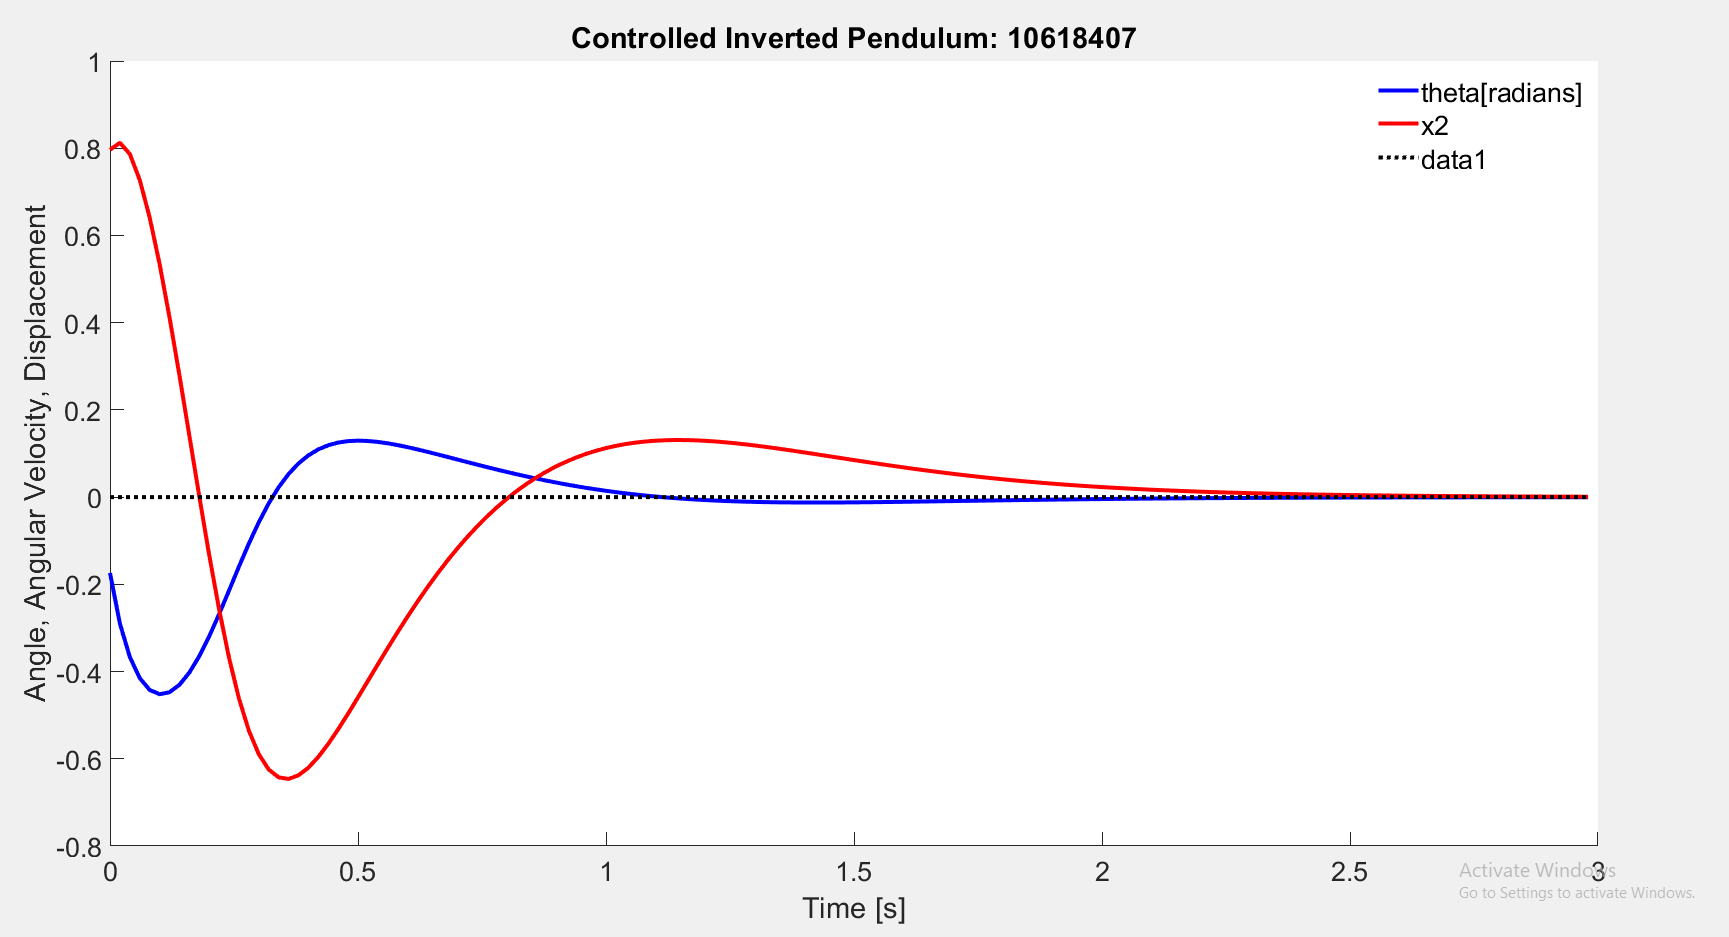
\includegraphics[width=12cm]{controlledPendulumOneKick.png}}
\caption{Single kick pendulum run with controlled poles}
\label{fig}
\end{figure}  

If the poles of the system are too small, as shown in fig.(2.4) below, the system will return back to its original position very slowly. This would slow down the response of the cart when the pendulum is falling. This is known as overdamping and is shown in the graph below:

\begin{figure}[H]
\centerline{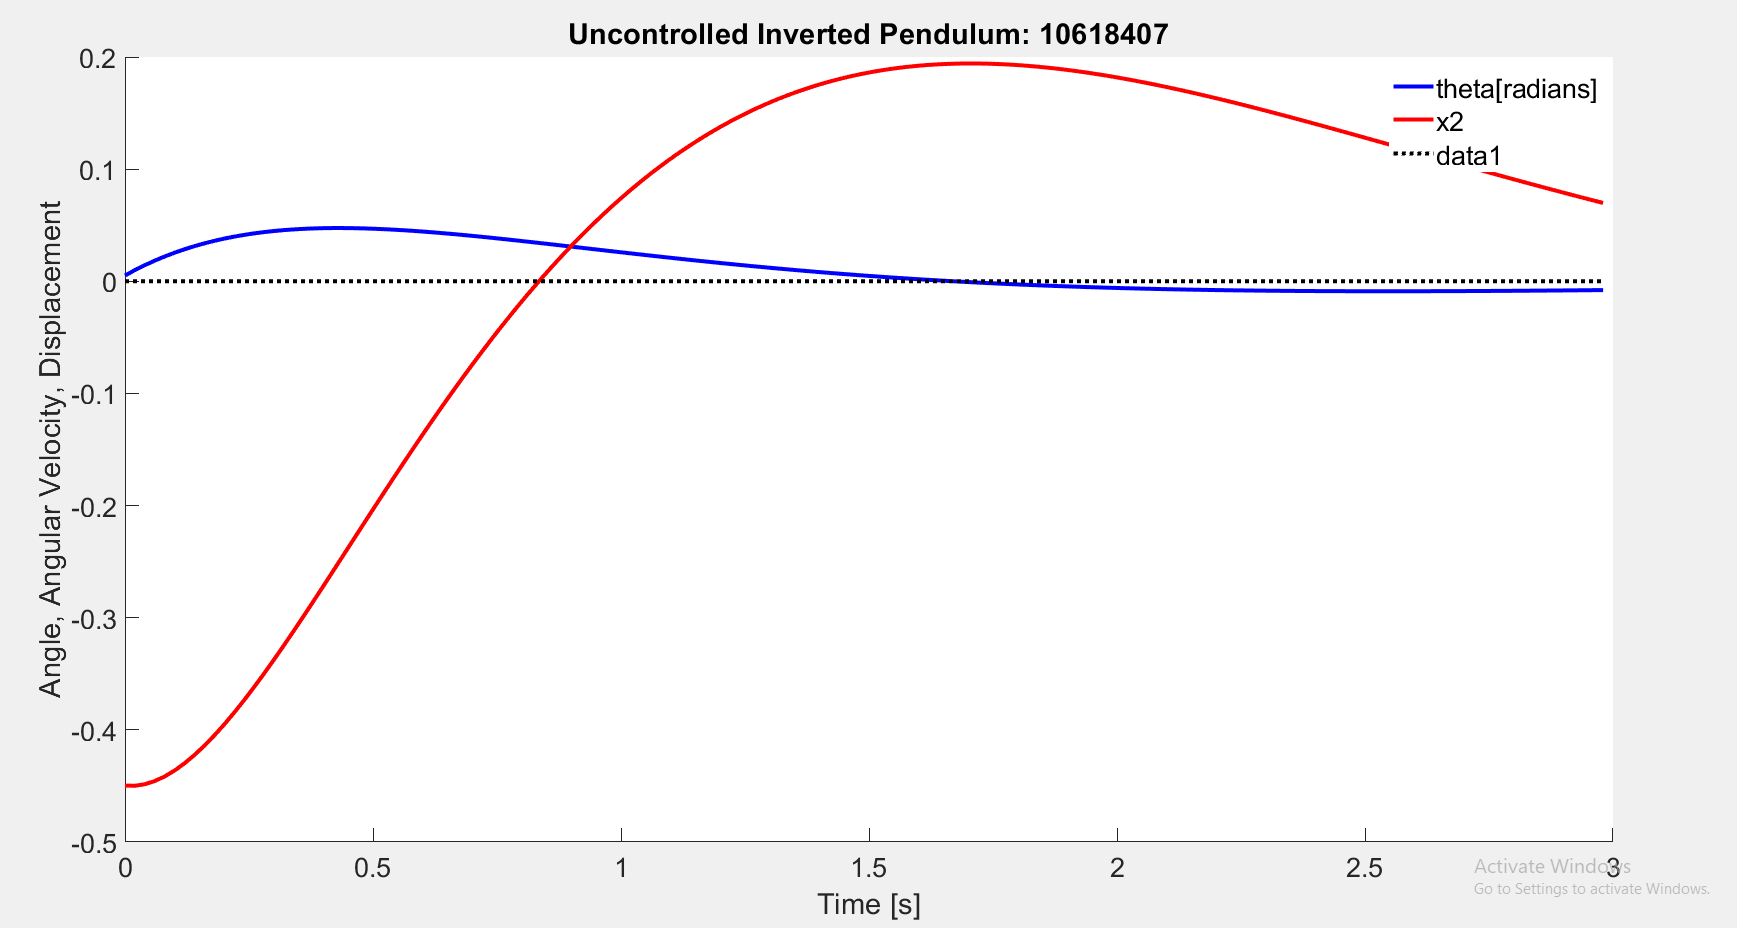
\includegraphics[width=12cm]{polesTooSmall.png}}
\caption{Initialisation code with poles that are too small}
\label{fig}
\end{figure}  

The poles to over damp the system were calculated using the code below:

\begin{figure}[H]
\centerline{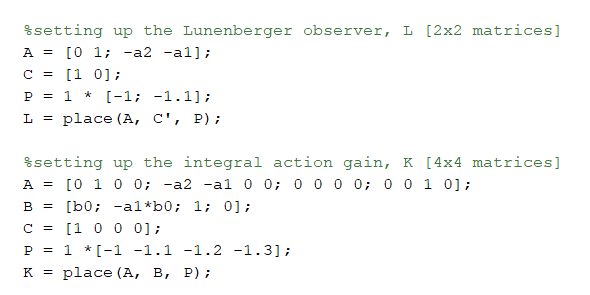
\includegraphics[width=12cm]{polesTooSmallCode.png}}
\caption{Single kick pendulum run with poles that are too small}
\label{fig}
\end{figure}  


If the poles of the system are too large, as shown in fig(2.6) below, the system will attempt to return to its original position too quickly. This is known as underdamping and will cause oscillation within the system. If these oscillations are not damped correctly, the system will become out of control because of the inherited instability of the controller with these pole values. In simulation, the pendulum and cart will travel to a distance nearing infinity. In reality, the cart will reach the end of the track and the pendulum will topple over. This is shown in the graph below:

\begin{figure}[H]
\centerline{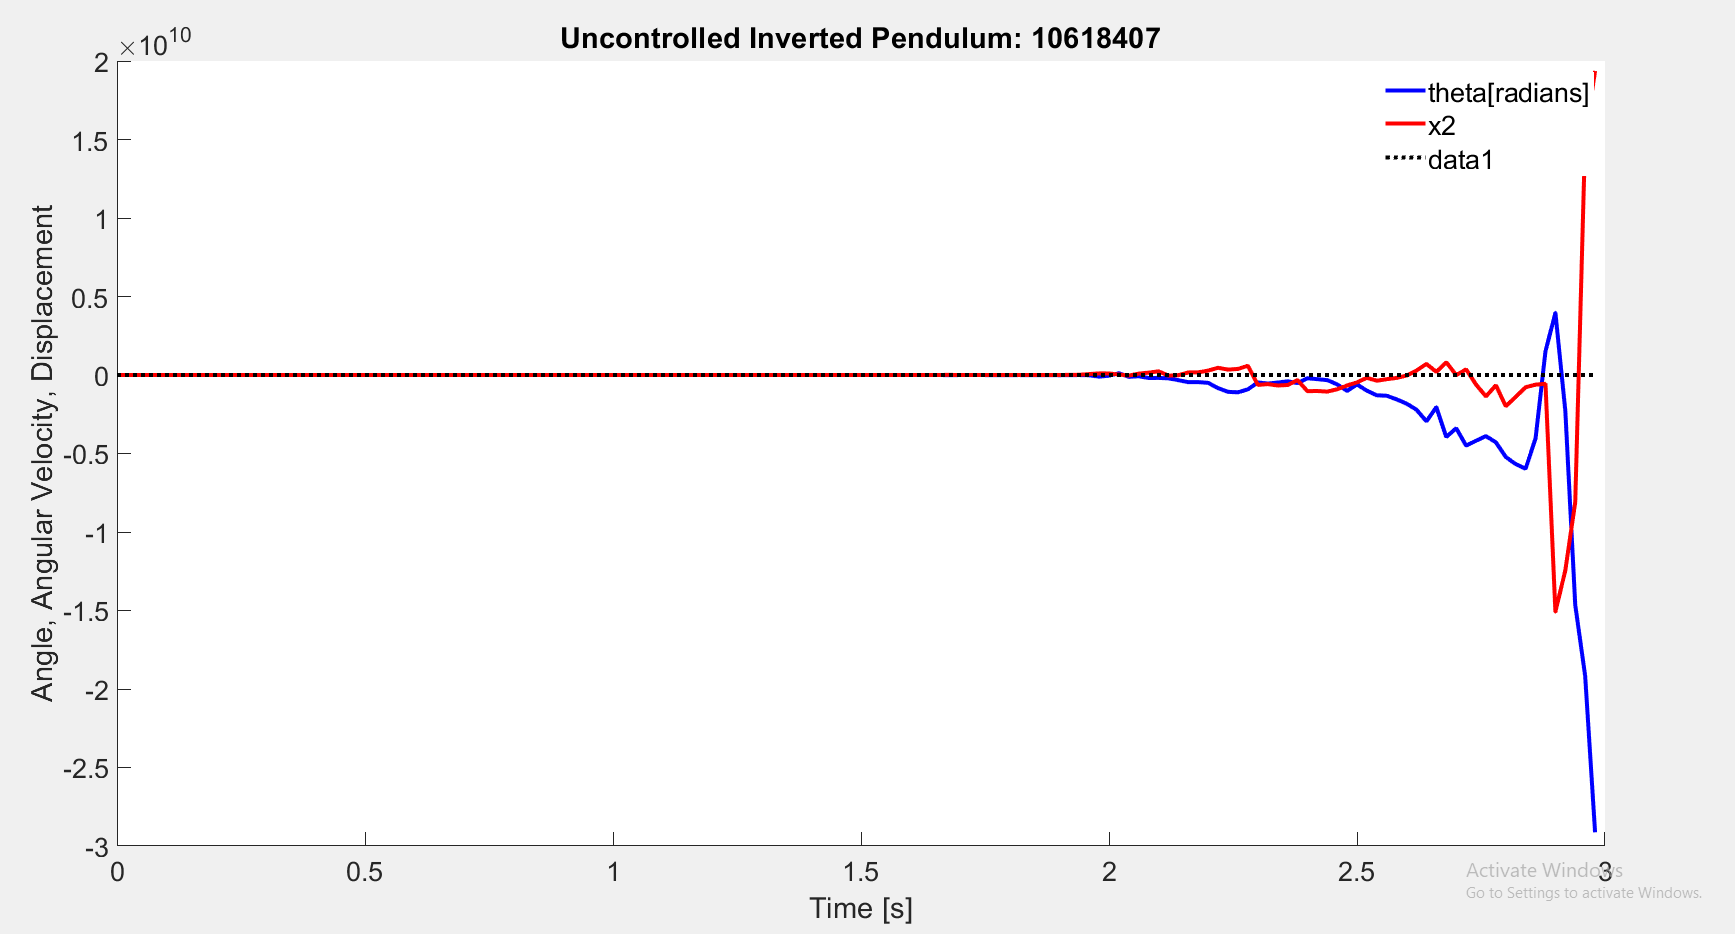
\includegraphics[width=12cm]{polesTooBig.png}}
\caption{Initialisation code with poles that are too large}
\label{fig}
\end{figure} 

The poles to under damp the system were calculated using the code below:

\begin{figure}[H]
\centerline{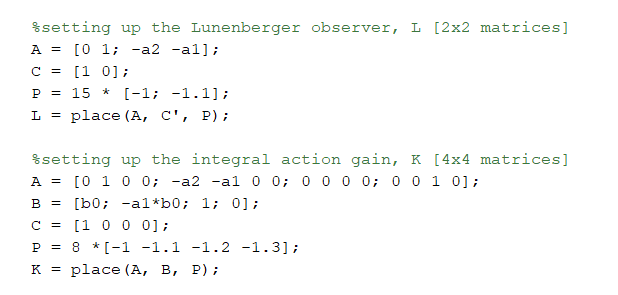
\includegraphics[width=12cm]{polesTooBigCode.png}}
\caption{Single kick pendulum run with poles that are too large}
\label{fig}
\end{figure}  

\subsubsection{Main Loop}

The variable `runs', at the top of the loop, determines how many times the code will run (how many times the pendulum is `kicked'). A pseudo-random set of initial conditions is generated for simulation purposes. If there were no initial conditions (all zero) the pendulum would remain perfectly upright, due to the noiseless nature of the simulation. The main loop is where the state space integrator function is called and run. The kick arrow is shown only at the start of each run so it does not obscure the view of the pendulum. The new data for each of the runs is concatenated with the old run. This is the data used for the animation, as shown in the code below: 

\begin{figure}[H]
\centerline{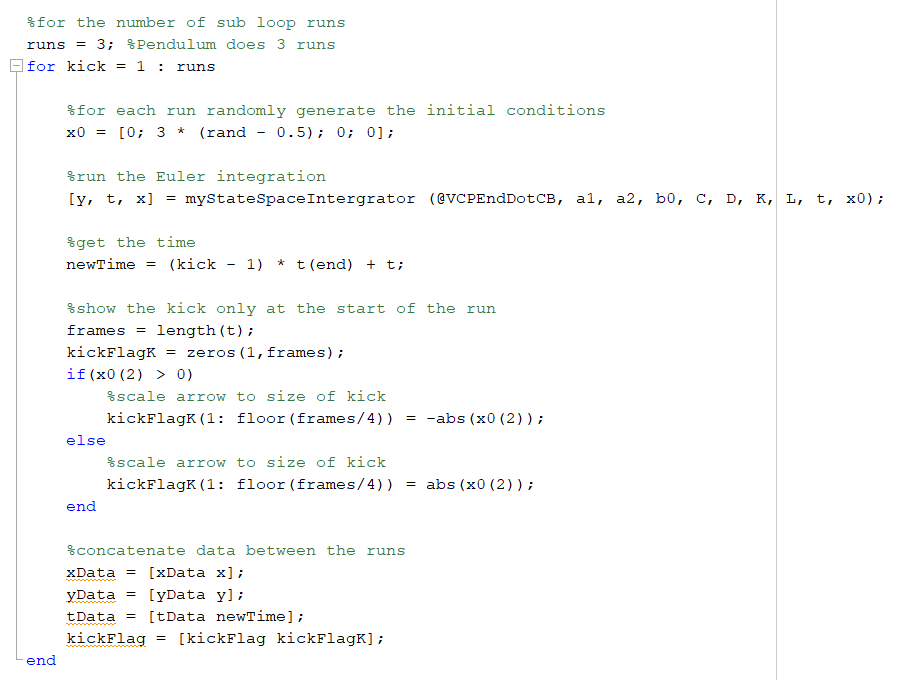
\includegraphics[width=12cm]{loopMain.png}}
\caption{Main loop for the pendulum code}
\label{fig}
\end{figure} 

\subsubsection{Plotting Values}

The plotting variables code is used to output all of the data points calculated in the loops into the various plot functions required to run the pendulum. This includes the title message for all the figures: 

\begin{figure}[H]
\centerline{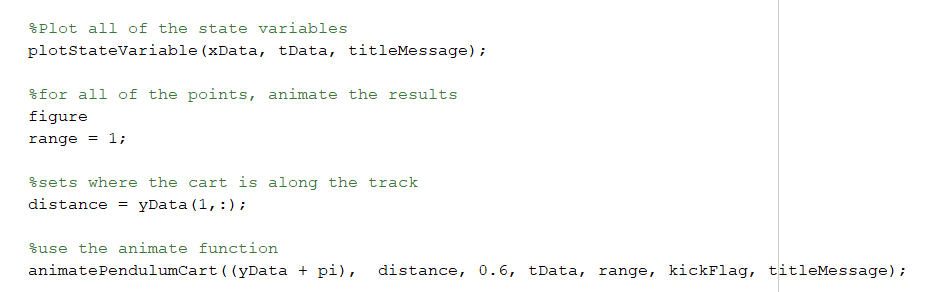
\includegraphics[width=12cm]{plotMain.png}}
\caption{Plotted values for the main pendulum code}
\label{fig}
\end{figure} 

The plot functions animatePendulumCart and plotStateVariable were given to us previously and have been unchanged for this project.

\subsection{State Space Integrator}  

The state space integrator is used to calculate the values for the state space model and the outputs $y$, $tout$, and $xout$. It is written in C-style, allowing the controller to be more easily implemented onto an Arduino or similar style microcontroller. This is useful for the real world implementation of the inverted pendulum. The loop inside the state space integrator is used to calculate the elements of the state space model for all of the frames of the animation. The state space integrator is shown in the figure below:

\begin{figure}[H]
\centerline{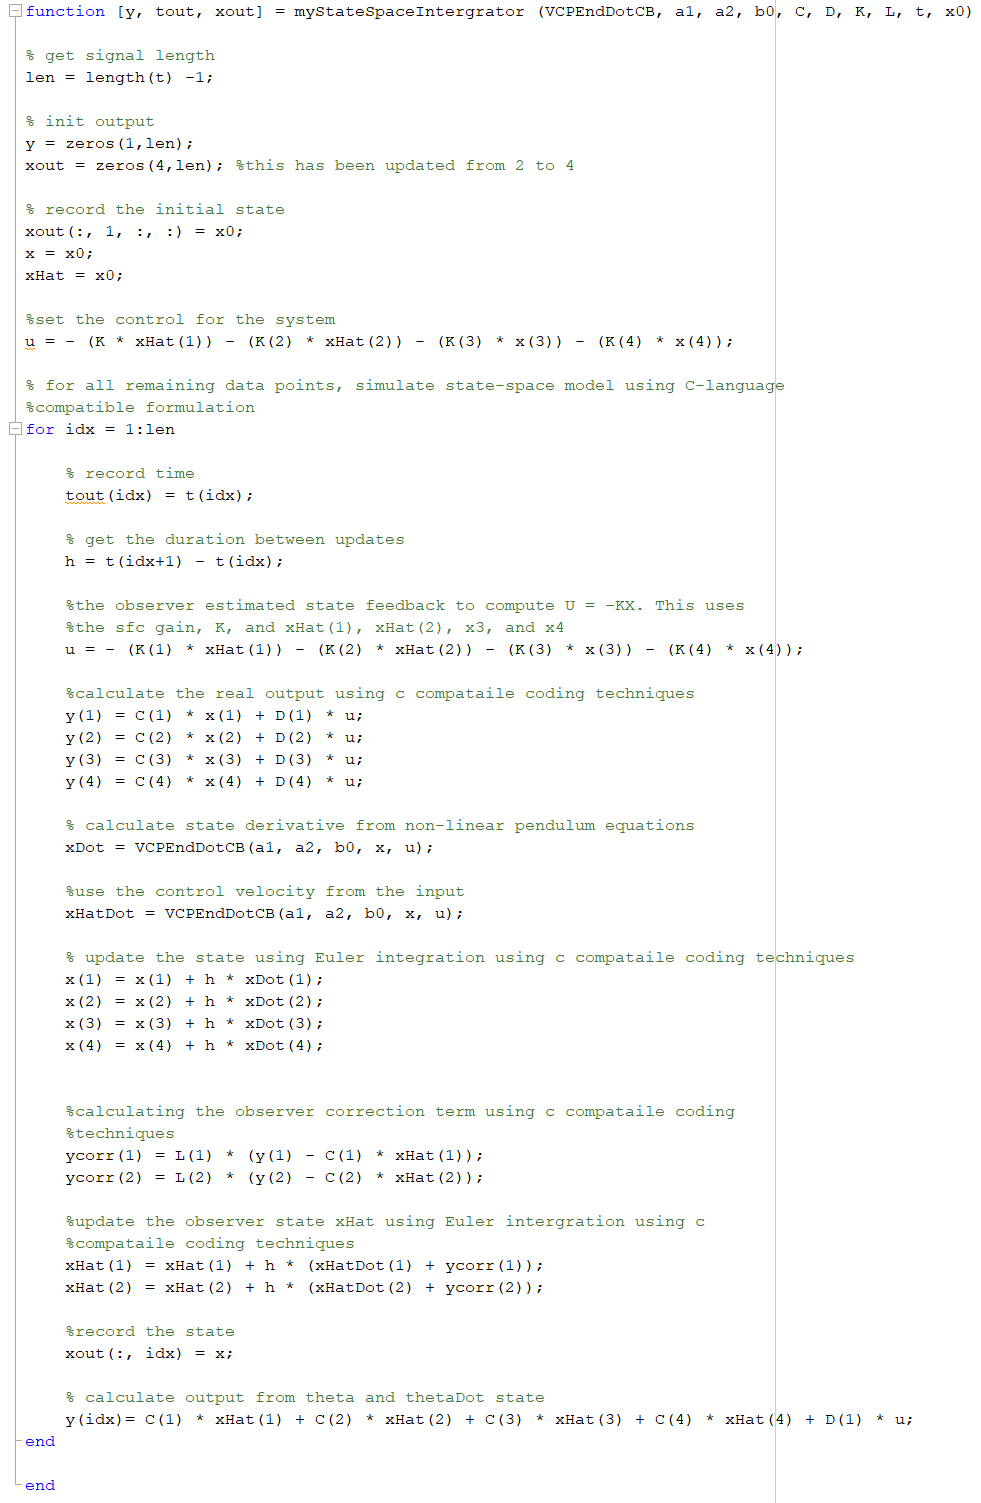
\includegraphics[width=12cm]{myStateSpaceIntergrator.png}}
\caption{State space integrator code for the inverted pendulum}
\label{fig}
\end{figure} 

\subsection{VCPendDotCB}

VCPendDotCB is called inside of the state space integrator code. It is used to calculate the values of $\dot{x}\textsubscript{1}$, $\dot{x}\textsubscript{2}$, $\dot{x}\textsubscript{3}$, and $\dot{x}\textsubscript{4}$. This is shown in the figure below:

\begin{figure}[H]
\centerline{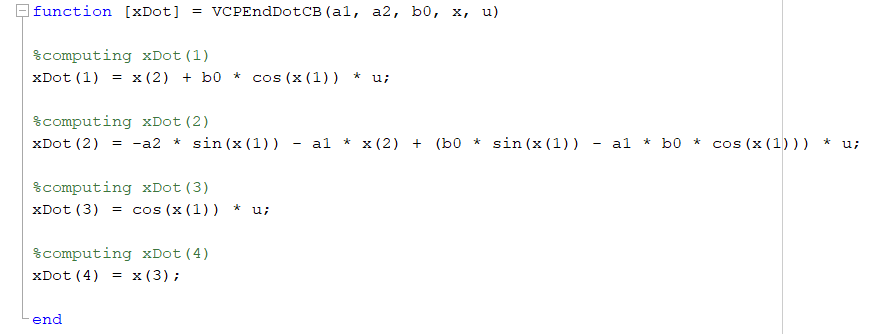
\includegraphics[width=12cm]{VCPEndDotCB.png}}
\caption{Output for the full state space place}
\label{fig}
\end{figure}

The output of VCPendDotCB is the matrix $\dot{x}$ which is passed back into the state space integrator function. 

\section{Run the Matlab simulation}

The simulation runs through all the frames for the pendulum. It displays a window that pops up onto the screen. This is the animation of the running pendulum, as shown in the figure below:

\begin{figure}[H]
\centerline{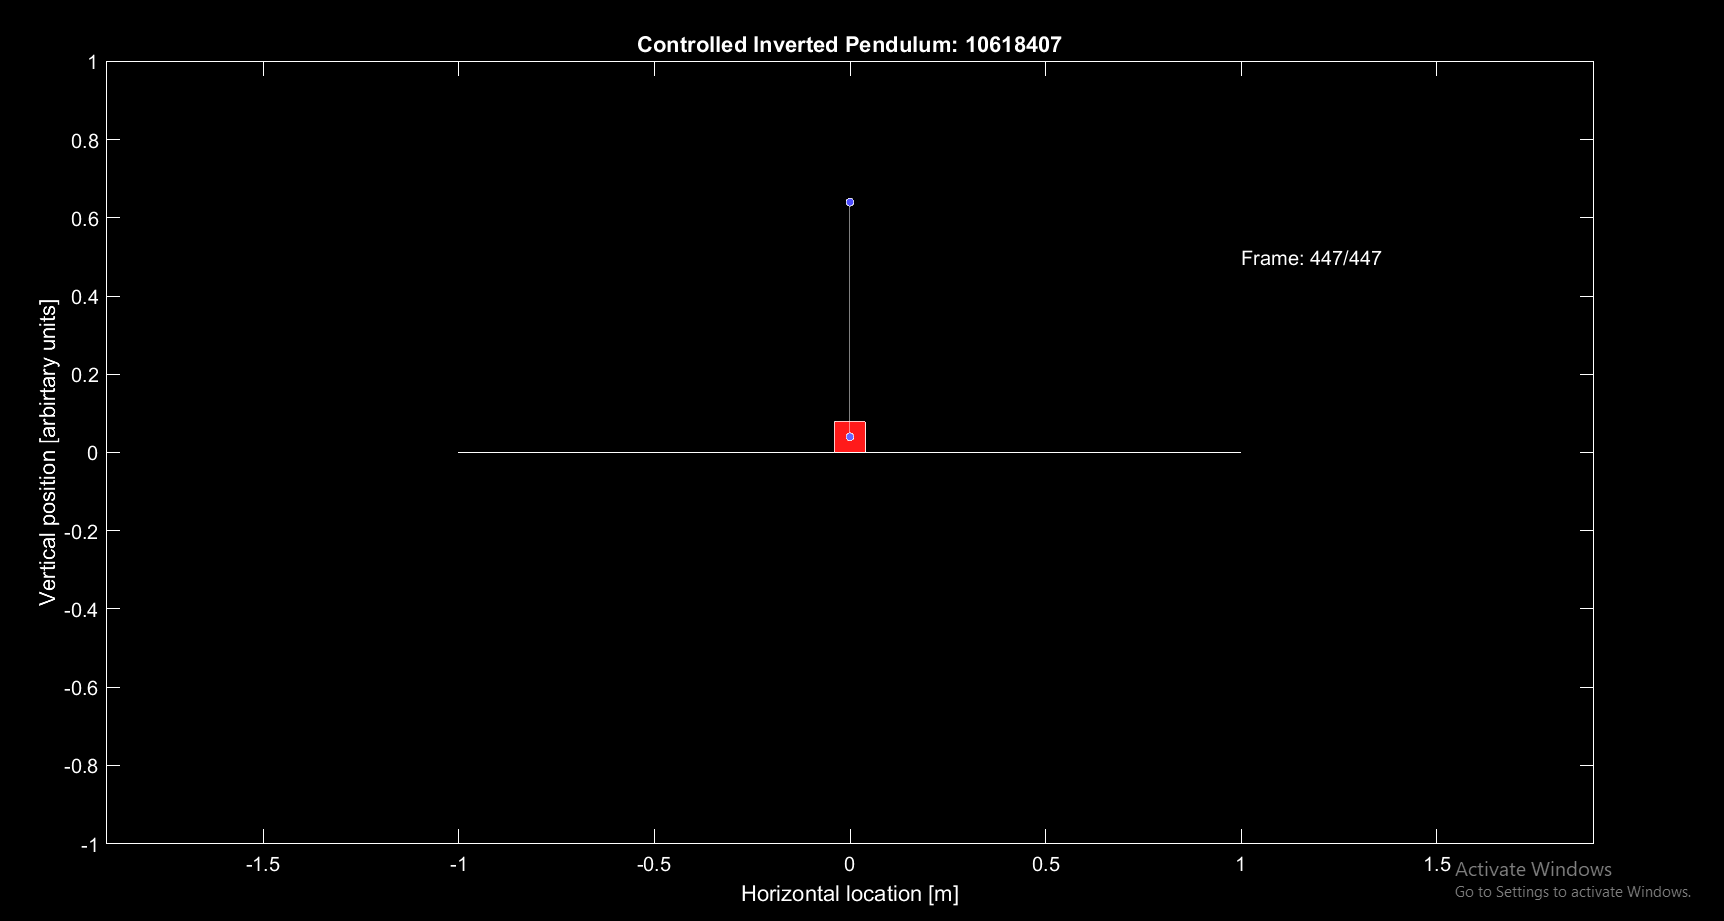
\includegraphics[width=12cm]{finalPendulumState.png}}
\caption{Final resting place of the inverted pendulum animation}
\label{fig}
\end{figure}

To see the animation of the inverted pendulum use the following link: \href{https://youtu.be/HhHBLydiXPE}{https://youtu.be/HhHBLydiXPE}\\

The figure below shows the relative motions of the pendulum in accordance to the angle, angular velocity, and displacement of the cart and pendulum arm. It is demonstrated that the oscillations of the inverted pendulum are damped heavily and the pendulum returns to its upright equilibrium state within two oscillations. The figure below shows the pendulum being controlled by the controller with effective critical damping:

\begin{figure}[H]
\centerline{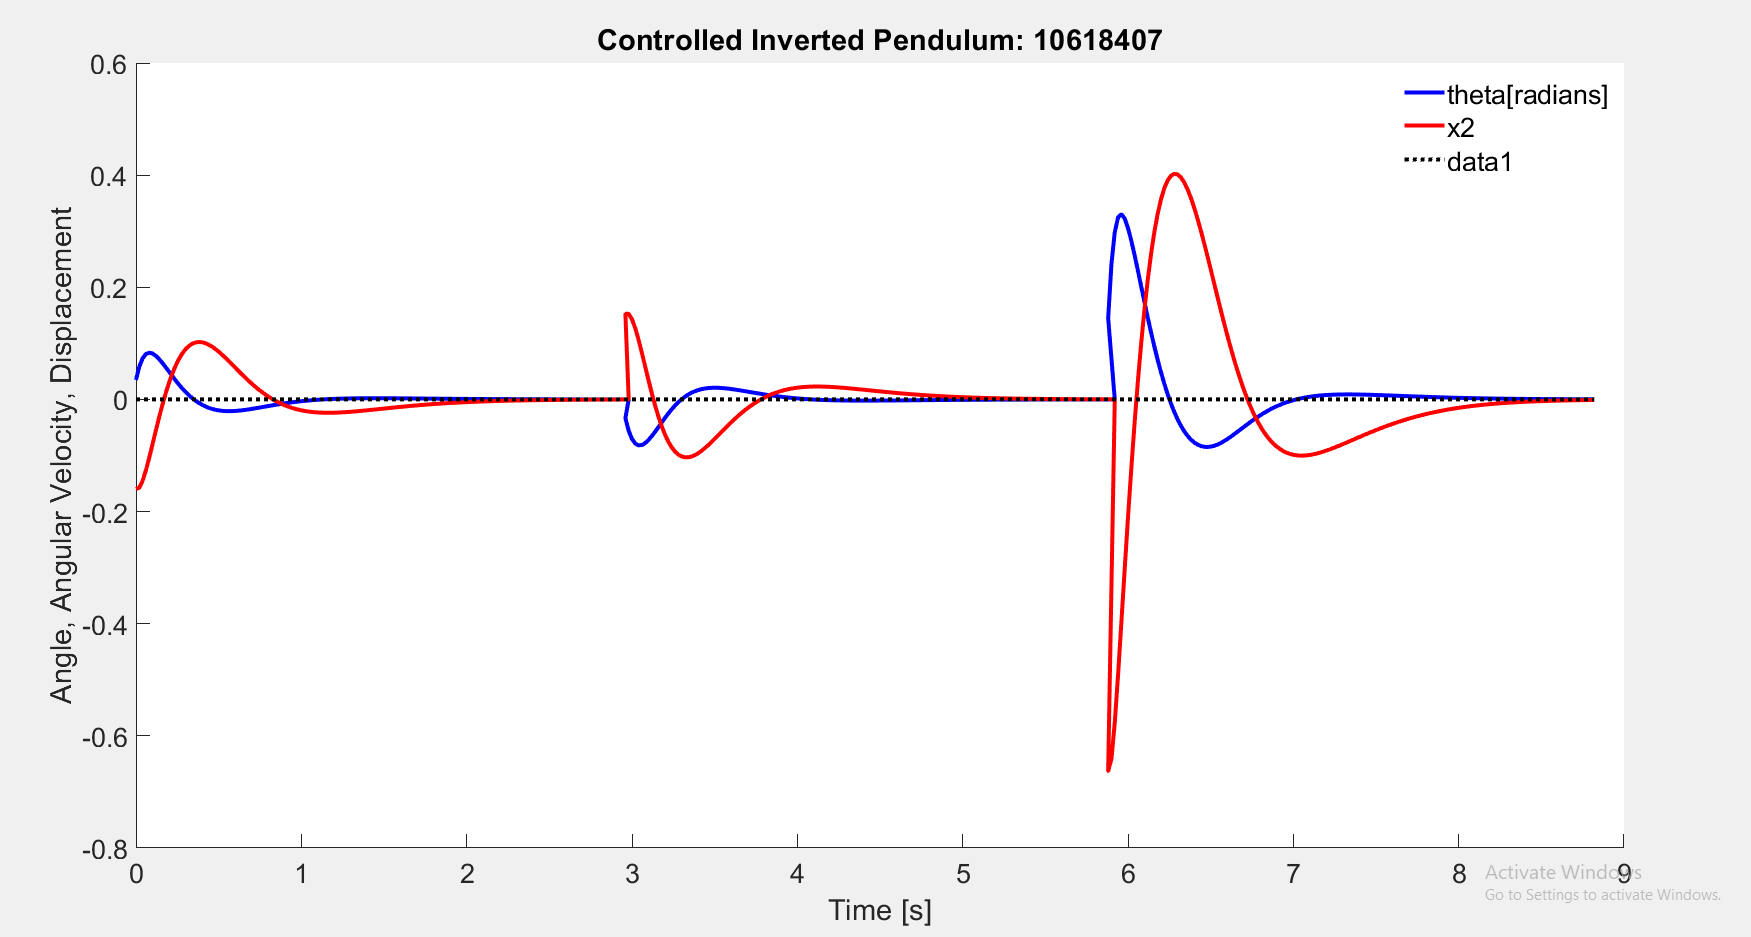
\includegraphics[width=12cm]{graphOfInvertedPendulum.png}}
\caption{The graph for the velocity of the inverted pendulum}
\label{fig}
\end{figure}

\end{document}